\documentclass[12pt]{report}

\usepackage[a4paper, left=2cm, right=2cm, top=2.5cm, bottom=2.5cm]{geometry}

\usepackage{tabularx}
\usepackage{amssymb}
\usepackage{amsmath}
\usepackage{graphicx}

\usepackage{minted}
\usepackage{adjustbox}
\usepackage{mdframed}
\usepackage{tcolorbox}
\usepackage{todonotes}
\usepackage{setspace}
\usepackage{hyperref}
\usepackage{caption}
\usepackage{abstract}
\usepackage{longtable}
\usepackage{array}
\usepackage[skip=20pt plus1pt, indent=40pt]{parskip}
\usepackage{biolinum}

\tcbuselibrary{skins,minted}

\usetikzlibrary{positioning,shapes,arrows}

\renewcommand{\familydefault}{\sfdefault}

% Set paragraph spacing
\setlength{\parskip}{4ex}

% Set line spacing
\onehalfspacing

\begin{document}

\begin{titlepage}
\begin{center}

\vspace*{1cm}
\makebox[\textwidth][c]{\includegraphics[width=0.5\textwidth]{pics/ime_usp_logo.png}}

\vspace{1cm}

\textbf{Universidade de São Paulo}
\textbf{Insitute of Mathematics and Statistics}
\textbf{Department of Computer Science}

\vspace{2cm}
\textbf{\LARGE Formal Methods for Validating Capitalization Tables and Transactions in the Venture Capital Market: Enhancing the Open Cap Table Format}

\vspace{2cm}

\textbf{\Large Rodrigo Ehrich Stevaux}

\vspace{1cm}

\textbf{\Large Advisor: Prof. Ana Cristina Vieira de Melo}

\vspace{3cm}
\begin{flushright}
\begin{minipage}{0.5\textwidth}
\begin{flushleft}
Dissertation presented to the Institute of Mathematics and Statistics at the University of São Paulo, as part of the requirements for the degree of Master of Science in Computer Science
\end{flushleft}
\end{minipage}
\end{flushright}

\vfill
\textbf{\large São Paulo}

\vspace{0.5cm}
\textbf{\large 2023}

\end{center}
\end{titlepage}

\newpage

\begin{abstract}
	This dissertation presents a model of the domain of startup financing, in particular a model for the transactions that compose to form capitalization tables. We present a recently released data interchange format (Open Cap Table format, or OCF) proposed by an industry coalition (Open Cap Table Coalition, or OCTC), and proceed to translate it from the original JSON Schema format to Alloy, a formal but lightweight specification language. We find that the Alloy model much more expressive and useful than the original JSON Schema, since it is more precise, captures subtle invariants in the  problem domain, and can be explored and checked with the Alloy Analyzer, which features model search and bounded model checking. Our research contributes to the field of formal methods as it shows how one can proceed from a semi-formal specification to a formal one, evaluates what the results, and contributes to the organization behind the data interchange format by providing a formal specification of their format.
\end{abstract}

\newpage

\tableofcontents

\thispagestyle{empty}
\listoffigures
\listoftables
\listoflistings
\listoftodos

\newpage
\pagenumbering{arabic}

\setcounter{chapter}{0}

\chapter{Introduction}

\section{Background and Motivation}

The venture capital market revolves around acquiring financial resources (capital for investment). This capital is invested in startup companies that the investor hopes will be sold for a large profit in the feature. It is an investment modality with high risk, but high returns. 

Startup companies obtain resources in stages that correspond to the progress made in achieving specific milestones. A funding round involves not only the startup itself and the investors, but an ecossystem of law firms, financial advisors and auditing firms. 

The transactions that take place in a funding round are complex, and the resulting data are difficult to maintain and validate. At each point in time in general, and immediately before and after a transaction, there is a relation between investors in the company and the number of shares they own (which might have different classes and rights). For any given company, the set of such relations at a given moment in time is commonly called a capitalization table.

Capitalization tables are typically kept in spreadsheets, and are exchanged frequently during negotiations. Given the limitations of spreadsheets, it is easy to make mistakes when updating them. This introduces risks of legal and financial liability, and can lead to disputes between investors and companies.

Giving the need for mitigating this risks, an ecossystem of software-as-a-service solutions has emerged to help companies manage their capitalization tables. However, these solutions are not interoperable, and there is no standard for exchanging capitalization table data.

The Open Cap Table Coalition\cite{opencaptablecoalitionOpenTable}, a recently formed alliance of key venture capital firms, law firms and software solution providers released what is a candidate for an industry standard for exchanging capitalization table data, known as the Open Cap Table Format\cite{OCTForma62:online} (which we will refer to as OCF). It is an open-source standard described semi-formally as schemas and validation rules for JavaScript Object Notation (JSON) documents. JSON is a popular data interchange format, and is used in many web applications. Specifically, the format follows the JSON Schema standard.

The OCF is a step forward in the direction of making capitalization tables reliable and easy to validate. However, it is not a formal specification, and it is inherently limited by the semantics of JSON Schema. A number of validations that emerge as constraints on the domain model, as we shall see, can not be captured by the semantics of JSON Schema, limiting the application of the format as a base for automated verification of the transactions that build a capitalization table.

\todo{Since in the research questions I have already given more specific results what we might expect, I can be more specific above}

In this thesis, we propose an alternative model for validating capitalization tables and transactions using the Alloy\cite{DJSALLA} language. Alloy is part of what is called lightweight formal methods, which are formal methods that are easier to use and require less training to apply than traditional formal methods (compared to other languages such as Z, B, TLA+)\cite{DJLMF}. It still allows sophisticated analysis of the constructed model. We show that the Alloy model is more expressive and useful than the original JSON Schema, since it is more precise, captures subtle invariants in the problem domain, and can be explored and checked with the Alloy Analyzer, which features model search and bounded model checking. 

\section{Research Questions and Contributions}

In this thesis, we explore the possibilities of using a language designed for formally expressing domains and concepts versus using a language designed for validating data structures. We use Alloy to model capitalization tables and transactions, and compare the results with the original JSON Schema model.

Given this setting, we aim to answer the following questions:

\begin{enumerate}
	\item Can Alloy be be used to assure that the model holds transactional integrity, that is, can it be used do defined the financial operations and constraints and ensure that they are consistent?
	\item Can the higher expressivity of Alloy be used to enhance the model's own expressivity, such as support for finer-grained business rules?
	\item What concepts can be expressed in Alloy that cannot be expressed on JSON Schema but are key for constraining the model to be more consistent with reality?
	\item Can we evaluate the results of the Alloy model in a way that is useful for the domain experts, and compare them to other forms of assuring correctness and realibity?
\end{enumerate}


\subsection{Contributions}

In investigating the research questions, we make the following contributions:

\begin{enumerate}
	\item We avoid double-issuances and double-spending of securities, as well as enforcing the correct order of transactions and the DAG-ness of the transaction graph
	\item We enhance the expressivity of business rules by explicitly modeling the AST that those rules would have if they where depicted as a domain-specific language
	\item We show how basic accounting equations can be checked for correctness over the resulting model, and how important queries can be specified and checked, such as querying for the complete history for a security, and show that those queries are correct
	\item We evaluate the output of Alloy Analyzer, that checks the models using a SAT solver, and includes parameters related to the size of the underlying bit-blasted model that can be compared to the coverage of regular unit tests
\end{enumerate}

\todo{In item 4, we have good references to quote from Ammans and Offutt, and we can also quote from the Alloy book}

Those are all properties that ultimately lie in legal contracts. Thus, our thesis helps bridge the gap between the ambiguities inherent to both natural language and the law, an important step into the development of accurate models of the domain, which is critical if we consider that having accurate and correct conceptual models is of paramount importante now to check the correctness of large language models and generative AI in general.

\todo{This is very powerful and must be emphasized elsewhere}

\todo{Bring a wealth of quotes from the media, showing how LLMs are exploding, and adding a more methodological note that events are unfolding as this is written}
\section{Thesis Organization}

The remainder of this thesis is organized as follows.

\todo{Complete this section with the organization of the thesis, after the rest of the thesis is written.}

In the appendix, the reader will find full code listings for the Alloy model, and the JSON Schema for the Open Cap Table Format, the grammar and description of JSON Schema and a quick reference for Alloy.


\chapter{Background}

This thesis is meant for the general computer science public, and so we will provide some background on the tools and technologies used in this thesis. We will also provide some background on capitalization tables and ecossystem of software solutions, including the OpenCapTable Format.

\section{Overview of Alloy and JSON Schema}

We use two languages in this thesis: Alloy and JSON Schema.

Alloy is a language for describing models in first-order logic and the Alloy Analyzer is a tool for analyzing such models. JSON Schema is a data validation format for JSON documents, with a JSON-based syntax.

\subsection{Overview of Alloy}

Alloy\cite{DJSALLA} is a formal specification language and analysis tool developed by Daniel Jackson and his colleagues at the Massachusetts Institute of Technology (MIT). Alloy allows users to define abstract models of complex systems and to automatically check their properties using a bounded model checking algorithm. Alloy's syntax is based on first-order logic and set theory, and includes constructs for defining relations, functions, and constraints.

\noindent An Alloy model consists of the following parts:

\begin{itemize}
	\item Signature declarations, labeled by a \verb|sig| keyword, introduce a set of \textit{atoms} and a set of \textit{fields} relating atoms. A signature is similar but more general than a SQL table, for example.
	\item Constraint declarations, introduced by the keywords \verb|fact|, \verb|fun|, and \verb|predicate|, that limit the possible instances of the model. Facts are assumed to always hold.  Functions are reusable, named expressions, that return a relation. Predicates are functions that must evaluate to a boolean.
	\item Assertion declarations, introduced by the keyword \verb|assert|, that establish constraints that are expected to hold as consequences of the facts. Assertions can be checked by the Alloy Analyzer using the \verb|check| command.
\end{itemize}

Using the \verb|run| and \verb|check| commands, the user can ask the Alloy Analyzer to find examples and counter examples to expressions (usually built up from predicates) in a given \textit{scope}. The scope determines how many atoms can be created in the model (by signature). A larger scope is populated by more instances, but takes longer to check.

\subsubsection{Advantages of Alloy}

One of the key benefits of Alloy is its ability to quickly generate and evaluate different scenarios and configurations, allowing designers to iteratively refine their models and identify potential issues.

Alloys' value proposition is to take the ideal of precise and expressive notation based on a tiny core of simple and robust concepts, but it replace basic analysis based on theorem proving with a fully automatic analysis with immediate feedback.\cite{DJSALLA}

\begin{figure}
\centering
\includegraphics[width=0.8\textwidth]{pics/alloy-analyzer.png}
\caption{Alloy Analyzer}\label{fig:alloy-analyzer}
\end{figure}

\subsubsection{Applications of Alloy}

Alloy has been used in a wide range of applications in computer science, including software engineering, database design, security analysis\cite{Carpio2021}\cite{Chen2006}, multi-agent negotiations \cite{Podorozhny}. It has also been applied to modeling beyond computer science such as a model for central bank policy\cite{Johnson2021}. A model of the same-origin-policy used in web browsers can be found in the 500 Lines or Less open-source book\cite{500Lines19:online}. Alloy$\ast$ is a higher-order extension of Alloy that can be used for program synthesis, since it supports higher-order quantification\cite{Milicevic2017}. $\alpha{Rb}y$ is an embedding of Alloy in Ruby\cite{Arby}.


\subsection{Overview of JSON Schema}

JSON Schema, a specification for JSON (JavaScript Object Notation) data, provides a systematic approach to define the structure and constraints of JSON data. JSON, a lightweight data interchange format, is ubiquitously employed in web applications and APIs due to its simplicity and readability. JSON Schema, utilizing a JSON-based syntax, allows developers to meticulously define the structure and constraints of JSON data. A comprehensive description of JSON Schema is provided in RFC8259\cite{RFC8259}.

The versatility of JSON Schema is evident in its extensive range of validation rules and constraints. These include, but are not limited to, data types, required fields, minimum and maximum values, and regular expressions. Furthermore, JSON Schema supports custom validation rules and extensions, thereby offering developers the flexibility to define their own rules and constraints. This feature significantly enhances the adaptability of JSON Schema to cater to diverse and specific requirements.

JSON Schema is a powerful tool that leverages the simplicity and readability of JSON, making it human-friendly and easy to comprehend. It employs hypermedia principles, allowing schemas to reference other schemas through a Universal Resource Identifier (URI). This feature enhances the modularity and reusability of schemas, thereby promoting efficient schema design and management.

In the context of designing messages for HTTP application programming interfaces (APIs), JSON Schema proves to be exceptionally adequate. It provides robust validation capabilities, ensuring the integrity and consistency of data communicated through APIs. Not only can it validate the presence of all necessary arguments, but it also offers basic format validation. This means it can check if the data conforms to the specified types, patterns, or other constraints, thereby ensuring that the data received or sent via APIs adheres to the expected structure and format. This comprehensive validation capability significantly enhances the reliability and robustness of HTTP APIs, making JSON Schema an indispensable tool in modern web development.

See table \ref{tab:json-schema-validation-keywords} for a list of validation keywords.

\begin{table}[h!]
\centering
	\begin{tabular}{|l|p{10cm}|}
		\hline
		\textbf{Validation Keyword} & \textbf{Description}                                                          \\
		\hline
		type                        & Specifies the data type (e.g., string, number, object, array, boolean, null)  \\
		\hline
		enum                        & Specifies a predefined list of acceptable values                              \\
		\hline
		const                       & Specifies a constant value that the data must match                           \\
		\hline
		multipleOf                  & Specifies that a numeric instance is divisible by this keyword's value        \\
		\hline
		maximum                     & Specifies the maximum numeric value                                           \\
		\hline
		exclusiveMaximum            & Specifies a numeric instance to be strictly less than this keyword's value    \\
		\hline
		minimum                     & Specifies the minimum numeric value                                           \\
		\hline
		exclusiveMinimum            & Specifies a numeric instance to be strictly greater than this keyword's value \\
		\hline
		maxLength                   & Specifies the maximum length of a string                                      \\
		\hline
		minLength                   & Specifies the minimum length of a string                                      \\
		\hline
		pattern                     & Specifies a regular expression that a string must match                       \\
		\hline
		items                       & Specifies constraints for array items                                         \\
		\hline
		maxItems                    & Specifies the maximum number of items in an array                             \\
		\hline
		minItems                    & Specifies the minimum number of items in an array                             \\
		\hline
		uniqueItems                 & Specifies that all items in an array must be unique                           \\
		\hline
		properties                  & Specifies constraints for object properties                                   \\
		\hline
		required                    & Specifies required properties in an object                                    \\
		\hline
		additionalProperties        & Specifies whether additional properties are allowed                           \\
		\hline
	\end{tabular}
\caption{Available Validations in JSON Schema}
\label{tab:json-schema-validation-keywords}
\end{table}
  
\subsubsection{Tooling for JSON Schema}

JSON Schema is supported by a large number of tools\cite{jsonschemaImplementations}: validators, schema generators and code generators. There are validators for all major languages, and the schema generators can generate schemas from code, data and models. Code generators can implement basic Web-based user interfaces and generate data based on schemas.

There is also a noteworthy repository of JSON Schemas for hundreds of APIs, called JSON Schema Store\cite{schemastoreJSONSchema}.

\subsection{Mapping from JSON Schema to Alloy}

Here we describe our general approach for translating JSON Schema into Alloy. Basically, we follow the steps:

\begin{figure}[ht!]
\centering
	\begin{minipage}{.8\linewidth}
		\begin{enumerate}
			\item\label{itm:abstract_signature} Translate the \textit{schemas} into \textit{abstract signatures} in Alloy, devoid of any fields.
			\item\label{itm:concrete_signature} Iterate over each \textit{abstract signature} from step \ref{itm:abstract_signature}. For each, instantiate it into a \textit{concrete signature} and incorporate the corresponding fields as specified in the JSON schema.
			\item\label{itm:related_signatures} Examine each field from step \ref{itm:concrete_signature}. Consequently, introduce the pertinent signatures into our \textit{stack} and return to step \ref{itm:concrete_signature}.
			\item\label{itm:assertions} Formulate \textit{assertions} which are anticipated to be upheld given the domain currently being modeled.
			\item\label{itm:analyzer} Employ the \textit{Alloy Analyzer} to assess whether the assertions from step \ref{itm:assertions} are satisfied. If not, progress to the subsequent step.
			\item\label{itm:constraint} Extend the Alloy model with a fresh \textit{constraint} if the assertions from step \ref{itm:assertions} were not satisfied. Repeat steps from \ref{itm:concrete_signature} to \ref{itm:constraint} until all assertions hold true.
		\end{enumerate}
	\end{minipage}
\caption{Process of creating an Alloy model from schemas}
\label{fig:json-to-alloy-translation-algorithm}
\end{figure}  

Our scheme implements a depth-first search of the original schema, and when completed, the Alloy model should be a roughly direct translation of the original schema. Once this is done, we can start improving the model using the more expressive semantics of Alloy, always checking if the assertions hold.

\section{What are Capitalization Tables?}

Formally, a capitalization table can be defined as a mapping of the set of stakeholders in a company to the number of shares they own in each asset class in the company. In this thesis we consider common stocks and stock options as asset classes. Mathematicall, assuming $S$ is the set of stakeholders, $A$ is the set of asset classes, a capitalization table at date $t$ is a function $C_t: S \times A \rightarrow \mathbb{N}$.

\subsection{Overview of Capitalization Tables}


A capitalization table is a snapshot of the relationship of stakeholders in a company and the number of shares they own in each asset class in the company. In this thesis we consider common stocks and stock options as asset classes.

\begin{table}[h!]
\centering
	\begin{tabular}{|l|l|l|l|l|}
		\hline
		Investor       & Asset Class     & Shares & Cost (USD) & \% of Company \\
		\hline
		Founders       & Common Stock    & 10,000 & -          & 71.43\%       \\
		Seed Investors & Preferred Stock & 2,000  & 2,000,000  & 14.29\%       \\
		Option Pool    & Common Stock    & 2,000  & -          & 14.29\%       \\
		\hline
		Total          & -               & 14,000 & 2,000,000  & 100.00\%      \\
		\hline
	\end{tabular}
\caption{Example of a capitalization table}
\label{tab:example-capitalization-table}
\end{table}

Here, the set of stakeholders $S$ is $\{ \text{Founders}, \text{Seed Investors}, \text{Option Pool} \}$, and the set of asset classes $A$ is $\{ \text{Common Stock}, \text{Preferred Stock} \}$. The capitalization table is a function $C: S \times A \rightarrow \mathbb{N}$, where $C(\text{Founders}, \text{Common Stock}) = 10,000$, $C(\text{Seed Investors}, \text{Preferred Stock}) = 2,000$, and so on.

Changes in a capitalization table are effects from transactions (both in the business sense, but also in the computing sense): issuance of shares to new investors, transfers of shares between investors, and formation of pools for and exercise of stock options by employees.

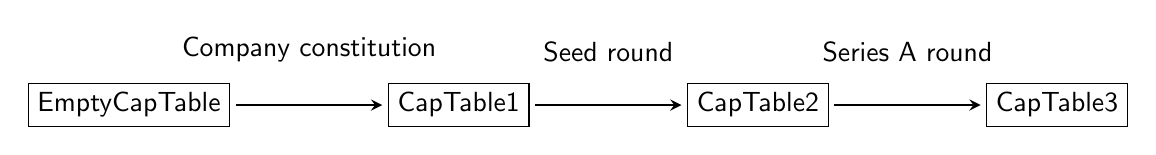
\begin{tikzpicture}[
    >=stealth,
    node distance=2cm,
    pil/.style={
        ->,
        thick,
        shorten <=2pt,
        shorten >=2pt,}
]
  
\node[rectangle,draw] (empty) {EmptyCapTable};
\node[rectangle,draw,right=of empty] (cap1) {CapTable1};
\node[rectangle,draw,right=of cap1] (cap2) {CapTable2};
\node[rectangle,draw,right=of cap2] (cap3) {CapTable3};
  
\path[pil] (empty) edge [above] node [yshift=12pt] {Company constitution} (cap1);
\path[pil] (cap1) edge [above] node [yshift=12pt] {Seed round} (cap2);
\path[pil] (cap2) edge [above] node [yshift=12pt] {Series A round} (cap3);
  
\end{tikzpicture}

\subsubsection{Why are Capitalization Tables Important?}

Cap tables are important for several reasons. First, they provide a clear and accurate picture of the ownership structure of the company, which is crucial for decision-making and financial reporting. Second, they help to ensure that equity is distributed fairly and transparently among shareholders. Finally, they can be used to calculate the potential payouts and returns for different scenarios, such as a sale of the company or an initial public offering (IPO). A venture capital firm may use a cap table to track the ownership and value of its portfolio companies. The cap table can help the firm to make informed decisions about future investments, and can help to identify potential exit opportunities.


Critically, the cap table can help to ensure that the ownership and value of the company is distributed fairly among investors and founders, and can help to identify potential issues or conflicts.

\subsubsection{How are Capitalization Tables Used?}

Here are the typical operations in startup financing. All have effects on the final capitalization table.

\begin{longtable}[h!]{|p{5cm} | p{8cm}|} 
\caption{Common startup financing operations} \\
	\hline
	\textbf{Operation}         & \textbf{Description}                                                                                           \\ [0.5ex] 
	\hline
	\endfirsthead
	
	\multicolumn{2}{c}%
	{\tablename\ \thetable\ -- \textit{Continued from previous page}} \\
	\hline
	\textbf{Operation}         & \textbf{Description}                                                                                           \\ [0.5ex]
	\hline\hline
	\endhead
	
	\hline \multicolumn{2}{r}{\textit{Continued on next page}} \\
	\endfoot
	
	\hline
	\endlastfoot
	
	Equity financing           & Money from investors is converted into shares at a given price-per-share                                       \\ 
	Convertible note financing & Money from investors is lent to the company as debt, but with a provision to convert into shares in the future \\ [1ex]
	Employee stock options     & Employees are given the right to purchase shares at a given price-per-share in the future                      \\ [1ex]
	\hline
\end{longtable}
\subsection{Examples}

\textbf{Seed round with convertible debt}

\vskip1cm

Here a new startup has only founders in its capitalization table. The founders have 10,000 shares. The company raises \$1,0M in a convertible note financing. The convertible note has a \$20M valuation cap. The convertible note converts into shares at the next equity financing round. Thus, shares can be given as actually issued shares and fully diluted shares, which are estimates based on corresponding schedule stock issuances.

\vskip1cm

\begin{center}
	\begin{tabular}{|p{3cm}|p{3cm}|p{3cm}|}
		\hline
		Shareholder  & Shares & Percentage \\
		\hline
		Founders     & 10,000 & 100\%      \\
		\hline
		Total        & 10,000 & 100\%      \\
		\hline
		Common Stock & 10,000 & 100\%      \\
		\hline
	\end{tabular}
	
\end{center}

\vskip1cm

\begin{center}
	\begin{tabular}{|p{3cm}|p{3cm}|p{3cm}|p{3cm}|}
		\hline
		Shareholder       & Shares   & Shares          & Percentage \\
		                  & (Actual) & (Fully Diluted) &            \\
		\hline
		Founders          & 10,000   & 10,000          & 95\%       \\
		\hline
		Investor I (Debt) & 0        & 526.32          & 5\%        \\
		\hline
		Total             & 10,000   & 10,526.32       & 100\%      \\
		\hline
	\end{tabular}
\end{center}

\subsubsection{Problems in managing capitalization tables}

Cap tables may change frequently, reflecting changes in ownership, investment, and valuation over time. They are complex to manage and validate, because they are only a snapshot, a state. A cap table can only be verified in trivial ways \- sums and percentages not adding up. 

But the financial operations and transactions that evolve a capitalization table must comply with a series of legal and business rules that are ultimately defined in business contracts, and software to do so must take into account the following:

\begin{enumerate}
	\item Avoid double spending and ensuring the overall life of a security is correct (it must be created once and spent only if ever created, and it can undergo non-terminal transactions)
	\item No cycles should be possible in the life cycle of any security (a security can not be both the input and output of a single transaction or a set of transactions such as a partial cancellation that creates a residual security)
	\item Support very complex business rules that are defined in business contracts, and that are not trivial even to specify
	\item Respect basic accounting equations such as that the number of shares in circulation must never exceed the number of shares created
\end{enumerate}

Which are reflected in our research questions.

\section{Ecossystem and The Open Cap Table Format}

In the last decade (2010-2020), a number of software-as-a-service solutions have emerged in the capitalization table management and related spaces in various geographies. These solutions are not interoperable, and there is no standard for exchanging capitalization table data.

The Open Cap Table Format (OCF) is a data interchange format for capitalization tables. It is a JSON Schema-based format that is designed to be easy to use and understand. The OCF is intended to be used by startups, investors, and other stakeholders in the venture capital market.

In the next chapter, we will give a detailed description of the OCF, and in the following chapters we will provide a translation of the most important parts of the OCF into an Alloy specification.

% Solutions in the space
% Carta, founded as eShares in 2012, specializes in capitalization table management, with reportedly 2.4M users and USD 2.5tn in assets in the platform.
% Shareworks, founded in 1999 and now owned by Morgan Stanley, manages capitalization tables and also offers compensation financial planning solutions for employees\cite{Sharewor68:online}.
% The Long-term Stock Exchange, is stock exchange founded in 2015 focused on long-term value creation, has a cap table management solution\cite{LTSEHome63:online} with reportedly 40,000 startup founders using it.
% Create a nice table: company, founded at and description
\begin{tabular}{|l|l|p{6cm}|}
\hline
\textbf{Company}                                 & \textbf{Founded} & \textbf{Geography} \\ \hline
Shareworks\cite{Sharewor68:online}               & 1999             & USA                \\ \hline
Carta\cite{CartaEqu70:online}                    & 2012             & USA                \\ \hline
Long-term Stock Exchange\cite{LTSEHome63:online} & 2015             & USA                \\ \hline
Raise\cite{Software0:online}                     & 2018             & Africa             \\ \hline
Distu\cite{DistuEqu4:online}                     & 2021             & Brazil             \\ \hline
\end{tabular}


\chapter{Open Cap Table Format}

The Open Cap Table format is composed of 143 JSON Schema documents, which are organized in 8 files.  The files are organized in a directory structure, which is shown below. Thus the files package objects defined in the JSON Schemas.

\begin{tabular}{|p{6cm}|p{6cm}|}
    \hline
    \textbf{Files (total 8)}
    \begin{itemize}
    \item Issuers file
    \item Manifest file
    \item Stakeholders file
    \item Stock classes file
    \item Stock legend templates file
    \item Stock option plans file
    \item Transactions file
    \item Vesting terms file
    \end{itemize}
      &   
    \textbf{Schemas (total 143)}
    \begin{itemize}
    \item Types
    \item Enums
    \item Objects
    \end{itemize} \\
    \hline
\end{tabular}

\noindent Our work is based on commit \verb|20f3ede62d1f5bdbef16ae1edfa98c34fbda2610|, from 2022-Dec-30.

\section{Objects, Types, and Enums}

In this section, we will explore the different categories within the data model, including objects, types, and enums. Each category plays a distinct role and contributes to the overall structure and functionality of the model.

\subsection{Types}

The \texttt{types} directory contains schema files that define various types used in the model. These types serve as the foundation for creating structured data elements within the model. They define the format and constraints for specific data elements, ensuring consistency and integrity.

For example, the \texttt{Numeric.schema.json} file defines the type for numeric values, while the \texttt{Date.schema.json} file defines the type for representing dates. Other types may include addresses, monetary values, fractions, and more. These types not only provide the structure for the data but also enable validation by specifying required properties and data formats.

A useful type, for example, is the Monetary type. It defines a Monetary value as document with a Numeric value and a Currency Code value:

\begin{listing}[!h]
\begin{minted}{json}
{
  "\$schema": "http://json-schema.org/draft-07/schema",
  "\$id": "https://opencaptablecoalition.com/schema/types/Monetary.schema.json",
  "title": "Type - Monetary",
  "description": "Type representation of an amount of money in a specified currency",
  "type": "object",
  "properties": {
    "amount": {
      "description": "Numeric amount of money",
      "\$ref": "https://opencaptablecoalition.com/schema/types/Numeric.schema.json"
    },
    "currency": {
      "description": "ISO 4217 currency code",
      "\$ref": "https://opencaptablecoalition.com/schema/types/CurrencyCode.schema.json"
    }
  },
  "additionalProperties": false,
  "required": ["amount", "currency"],
  "\$comment": "Copyright © 2022 Open Cap Table Coalition (https://opencaptablecoalition.com) / Original File: https://github.com/Open-Cap-Table-Coalition/Open-Cap-Format-OCF/tree/v1.0.0/schema/types/Monetary.schema.json"
}
\end{minted}
\caption{The Monetary type}
\label{lst:monetary}
\end{listing}


\subsection{Enums}

The \texttt{enums} directory contains schema files that define enumerations within the model. Enums are used to represent a predefined set of values or options for specific properties. They provide a limited and consistent set of choices that can be assigned to certain attributes within objects.

For instance, the \texttt{TerminationWindowType.schema.json} file defines different types of termination windows, such as "Termination for Cause" or "Termination without Cause." Enums help to standardize and control the possible values for specific attributes, ensuring data consistency and providing a clear set of options to choose from.

\begin{listing}[!h]
\begin{minted}{json}
{
"$schema": "http://json-schema.org/draft-07/schema",
"$id": "https://opencaptablecoalition.com/schema/enums/TerminationWindowType.schema.json",
"title": "Enum - Termination Window Type",
"description": "Enumeration of termination window types",
"type": "string",
"enum": [
  "VOLUNTARY\_OTHER",
  "VOLUNTARY\_GOOD\_CAUSE",
  "VOLUNTARY\_RETIREMENT",
  "INVOLUNTARY\_OTHER",
  "INVOLUNTARY\_DEATH",
  "INVOLUNTARY\_DISABILITY",
  "INVOLUNTARY\_WITH\_CAUSE"
],
}
\end{minted}
\caption{The Termination Window Type enum}
\label{lst:termination-window-type-enum}
\end{listing}


\subsection{Objects}

The \texttt{objects} category represents the entities or concepts within the data model. Objects are composed of properties, which describe the attributes or characteristics of the entity they represent. Examples of objects include issuers, stakeholders, securities, and transactions.

Objects serve as the core components of the model, encapsulating both the data and behavior related to specific entities. They allow for the representation of real-world concepts and enable the modeling of relationships and interactions between different entities.

As an example, we show the Issuer type (abriged):

\begin{listing}[!h]
\begin{minted}{json}
{
    "$schema": "http://json-schema.org/draft-07/schema",
    "$id": "https://opencaptablecoalition.com/schema/objects/Issuer.schema.json",
    "title": "Object - Issuer",
    "description": "Object describing the issuer of the cap table (the company whose cap table this is)",
    "type": "object",
    "allOf": [
        {
            "$ref": "https://opencaptablecoalition.com/schema/primitives/objects/Object.schema.json"
        }
    ],
    "properties": {
        "object_type": {
            "const": "ISSUER"
        },
        "tax_ids": {
            "title": "Issuer - Tax ID Array",
            "description": "The tax ids for this issuer company",
            "type": "array",
            "items": {
                "$ref": "https://opencaptablecoalition.com/schema/types/TaxID.schema.json"
            }
        },
        "email": {
            "description": "A work email that the issuer company can be reached at",
            "$ref": "https://opencaptablecoalition.com/schema/types/Email.schema.json"
        },
        "phone": {
            "description": "A phone number that the issuer company can be reached at",
            "$ref": "https://opencaptablecoalition.com/schema/types/Phone.schema.json"
        },
        "address": {
            "description": "The headquarters address of the issuing company",
            "$ref": "https://opencaptablecoalition.com/schema/types/Address.schema.json"
        },
        "id": {},
        "comments": {}
    },
    "required": ["legal_name", "formation_date", "country_of_formation"],
}
\end{minted}
\caption{The Issuer object}
\label{lst:issuer-object-json-schema}
\end{listing}


By understanding the distinctions between objects, types, and enums, we gain a clearer perspective on the overall structure and purpose of the data model. These categories work together to define the data elements, provide validation, restrict attribute values, and represent the entities within the model.

\section{File Structure}
\subsection{OCF Manifest File}

The \texttt{OCF Manifest File} packages all data in a single artifact (a JSON file). Indeed, the OCF represents a data model, that is kept in files, which are collections of JSON documents. It is this file that is to be exchanged by the parties involved in the transactions.

The \texttt{OCFManifestFile} contains the following components:

\begin{tabular}{|l|l|l|}
    \hline
    \textbf{File}               & \textbf{Description}                      \\ \hline
    Issuer                      & The issuer of the securities.             \\ \hline
    Stakeholders file           & A file containing stakeholders.           \\ \hline
    Stock classes file          & A file containing stock classes.          \\ \hline
    Stock legend templates file & A file containing stock legend templates. \\ \hline
    Stock plans file            & A file containing stock plans.            \\ \hline
    Transactions file           & A file containing transactions.           \\ \hline
    Valuations file             & A file containing valuations.             \\ \hline
    Vesting terms file          & A file containing vesting terms.          \\ \hline
\end{tabular}

\subsection{Stakeholders File}

Contains stakeholders, which are persons or organizations that own securities. Stakeholders are assigned to securities in issuance transactions.

\subsection{Stock Classes}

Contains stock classes, which are types of securities. Stock classes can be preferred or common. Preferred stock classes gives the stakeholder certain rights, and preferred stock securities can usually be converted to common stock securities.

\subsection{Stock Legend Templates}

Contains stock legend templates, which are templates for stock legends. Stock legends are text that is printed on the stock certificate.

\subsection{Stock Plans}

Contains stock plans, which are pools for granting stock options to employees. Stock options give the right but not the obligation to buy a certain amount of stock at a certain price, and as the stock appreciates, the stock options become more valuable. Stock option plans are a key instrument in startup financing.

\subsection{Transactions File}

Contains transactions, which can be initial, non-terminal and terminal. Initial transactions are transactions that create securities. Non-terminal transactions are transactions that accept or adjust securities, including vesting events and exercises. If a non-terminal transaction generates a security, a matching initial transaction must be present. Terminal transactions are transactions that terminate securities, including sales and transfers.

\begin{tabular}{|l|c|c|c|c|}
    \hline
    \textbf{Transaction Type}       & \textbf{Convertible} & \textbf{PlanSecurity} & \textbf{Stock} & \textbf{Warrant} \\
    \hline
    Acceptance                      & Yes                  & Yes                   & Yes            & Yes              \\
    \hline
    Cancellation                    & Yes                  & Yes                   & Yes            & Yes              \\
    \hline
    ClassAuthorizedSharesAdjustment &                      &                       & Yes            &                  \\
    \hline
    ClassConversionRatioAdjustment  &                      &                       & Yes            &                  \\
    \hline
    ClassSplit                      &                      &                       & Yes            &                  \\
    \hline
    Conversion                      & Yes                  &                       & Yes            &                  \\
    \hline
    Exercise                        &                      & Yes                   &                & Yes              \\
    \hline
    Issuance                        & Yes                  & Yes                   & Yes            & Yes              \\
    \hline
    PlanPoolAdjustment              &                      &                       & Yes            &                  \\
    \hline
    Reissuance                      &                      &                       & Yes            &                  \\
    \hline
    Release                         &                      & Yes                   &                &                  \\
    \hline
    Repurchase                      &                      &                       & Yes            &                  \\
    \hline
    Retraction                      & Yes                  & Yes                   & Yes            & Yes              \\
    \hline
    Transfer                        & Yes                  & Yes                   & Yes            & Yes              \\
    \hline
\end{tabular}

\subsection{Valuations}

Contains valuations, which are observations of the value of the company. Valuations are used to calculate the value of securities.

\subsection{Vesting Terms}

Contains vesting terms, which are the representation of legal documents that define schedules for vesting events. Vesting events are events that cause securities to vest, which means that the securities become unrestricted and can be sold or transferred.

Vesting terms form a small domain-specific language for describing vesting schedules. The OCF can model both event-based vesting and time-based vesting. Event-based vesting is when vesting events are triggered by events, such as the company being acquired. Time-based vesting is when vesting events are triggered by time, such as the passage of time.

\section{Tracing Security Transactions}

In this section, we will explore the process of tracing security transactions within the data model. Tracing security transactions is crucial for accurately tracking the ownership and movement of securities throughout their lifecycle.

The case below shows the story of a single security, as traced by the transactions:

\begin{enumerate}\label{list:transactions}
	\item Issuance Event: 1,000 shares of preferred stock are issued to Bob (generates a new security id)
	\item Acceptance Event: Bob accepts the shares (refers to the security id generated in transaction 1)
	\item Conversion Event: Bob converts 500 shares to common stock (refers to the security id generated in transaction 1)
	      \subitem Since this is a partial transaction, beyond issuing a security for 500 shares of common stock, we must issue new preferred stock for the remaining 500 shares as well.
	\item \begin{enumerate}
	\item Issuance Event: 500 shares of common stock are issued to Bob (a new security id is generated)
	\item Issuance Event: 500 shares of preferred stock issued to Bob (a new security id is generated)
\end{enumerate}
\item Transfer Event: Bob transfers 500 shares of preferred stock to Alice
\subitem Again, this is a partial transaction, so we must issue new preferred stock for the remaining 500 shares as well.
\item \begin{enumerate}
\item Issuance Event: 500 shares of preferred stock are issued to Frank (a new security id is generated)
\item Issuance Event: 500 shares of preferred stock issued to Bob (a new security id is generated)
\end{enumerate}
\item Repurchase Event: Issuer repurchases 500 shares of common stock from Bob (This is a complete transaction, so no new security id is generated)
\end{enumerate}

Each of those transactions has a \verb|security_id| field. Securities, in the OCF, are correlation identifiers for tracing transactions. By querying the transactions file for all transactions refering to a given security id, we can trace the history of a security.

%%%%%%%%%%%%%%%%%%%%%%%%%%%%%%%%%%%%%%%%%%%%%%%%%%%%%%%%%%%%%%%%%%%%%%%%%%%%%%%%%%%%%%%%%%%%%%%%%%%%

\begin{listing}[!h]
\begin{minted}{json}
{
	"$id": "objects/transactions/issuance/StockIssuance.schema.json",
	"type": "object",
	"allOf": [
		{
		"$ref": "primitives/objects/Object.schema.json"
		},
		{
		"$ref": "primitives/objects/transactions/Transaction.schema.json"
		},
		{
		"$ref": "primitives/objects/transactions/SecurityTransaction.schema.json"
		},
		{
		"$ref": "primitives/objects/transactions/issuance/Issuance.schema.json"
		}
	],
	"properties": {
		"object_type": {
		"const": "TX_STOCK_ISSUANCE"
		},
		"stock_class_id": {
		"type": "string"
		},
		"share_numbers_issued": {
		"type": "array",
		"items": {
			"$ref": "types/ShareNumberRange.schema.json"
		}
		},
		"share_price": {
		"$ref": "types/Monetary.schema.json"
		},
		"quantity": {
		"$ref": "types/Numeric.schema.json"
		},
		"vesting_terms_id": {
		"type": "string"
		},
		"cost_basis": {
		"$ref": "types/Monetary.schema.json"
		},
		"stock_legend_ids": {
		"type": "array",
		"items": {
			"type": "string"
		}
		},
		"id": {},
		"comments": {},
		"security_id": {},
		"date": {},
		"custom_id": {},
		"stakeholder_id": {},
		"board_approval_date": {},
		"consideration_text": {},
		"security_law_exemptions": {}
	},
	"additionalProperties": false,
	"required": [
		"stock_class_id",
		"share_price",
		"quantity",
		"stock_legend_ids"
	]
}
\end{minted}
\caption{Stock Issuance Transaction}
\label{listing:stockissuance-transaction-json-schema}
\end{listing}



%%%%%%%%%%%%%%%%%%%%%%%%%%%%%%%%%%%%%%%%%%%%%%%%%%%%%%%%%%%%%%%%%%%%%%%%%%%%%%%%%%%%%%%%%%%%%%%%%%%%

Transactions might also have two additional fields: \verb|balancing_security _id| and \verb|resulting_security_ids|. Partial transactions such as partial cancellations and partial transfers effectively destroy the original security, and balances are kept in a new balancing security. Transfers also create new securities, so they have a \verb|resulting_security_ids| field.

\todo{Show how transactions can create securities, and how cancellations and transfers use a balancing security to allow partial cancellations and partial transfers, as a chain of transactions}

Thus the general form of a transaction, in the OCF, is:

\todo{Figure in tikz showing one output entering a box with two outputs}

\todo{Give a picture of transactions as inputs coming in, outputs coming out, and outputs are balancing and resulting securities}

Here limitations of JSON Schema appear: 
  

\textbf{Thus, in principle, the transaction tracing system which is a key enabler of auditability, can not be validated completely within the current implementation in JSON Schema.}

\begin{tabular}{|p{5cm}|p{8cm}|}
\hline
\textbf{Constraint}                                & \textbf{Explanation}                                                                                                                                                                                                           \\
\hline
Ordering of transactions                           & Transactions must appear in a certain order and must be linked by their security ids. JSON Schema cannot express this constraint, at least not naturally\footnotemark.                                                         \\
\hline
Balancing of transactions                          & The sum of shares entering and exiting a transaction must be balanced. JSON Schema can not perform arithmetic checks.                                                                                                          \\
\hline
(Non-)cyclicality of the implied transaction graph & More subtly, the graph formed by transactions can not be checked for cycles. This is a problem because cycles in the graph of transactions would mean that a security is being created out of thin air, which is not possible. \\
\hline
\end{tabular}
\footnotetext{We have not ruled out the possibility that such constraint could be encoded in JSON Schema some how.}

\section{Vesting Terms}

In this section, we show how the vesting terms define the conditions and schedules for the gradual vesting of securities. Here, the OCF is immensely valuable for accomodating the complexity of vesting terms, which are usually defined in legal documents.

\subsection{Vesting transactions}

\noindent\todo{Give the transactions for the vesting systems}
\subsection{Vesting objects, types and enums}

\noindent\todo{types and enums involved in vesting transactions}

\subsection{The DSL embedded in the vesting system}

\noindent\todo{Show the composition of vesting terms, vesting conditions and vesting triggers}

\todo{Argue that this is a domain-specific language embedded in the OCF}

\textbf{This is clearly a (proto-)domain specific language for vesting terms, which is embedded in the OCF. As we will develop in the following chapters, this idea of a DSL can be expanded to accomodate even more complex vesting terms, by introducing propositional logic operators and more date operators.}

\todo{Give the examples that appear in the OCF website}

\subsection{Useful types and enums in the vesting system}

Beyond the way that the vesting terms compose, the OCF also provides useful types for specifying dates, rounding methods and quantities that can be given as percentages, fractions or absolute values.

\todo{Show how quantities can be modelled using fractions and etc, show a few of the date types and rounding enums}

\section{Conversion Mechanisms}

In this section, we show how conversion mechanisms enable the transformation of securities from one type to another, which usually involves either the conversion of preferred stock into common or the conversion of debt into equity.

\subsection{Conversion transactions}

\noindent\todo{Give the transactions for the conversion systems}

\subsection{Conversion objects, types and enums}

\noindent\todo{types and enums involved in conversion transactions}

\subsection{The conversion process}

\todo{Show how conversion always means consuming a security in exchange for another in another class, still respecting security tracing}

\todo{Show how complex it is to define the rules for conversion, because they carry uncertainty \- convertible debt can convert into equity at a given ratio but also convert into a fixed percentage of the company's ownership, regardless of the valuation}

\section{Evaluation of the Data Model}

\subsection{Review of the building blocks}

In this chapter, we showed how the OCF is based upon:

\begin{itemize}
	\item \textbf{Transactions} and their tracing, which are the basic operations that can be performed on securities;
	\item \textbf{Vesting terms}, which are the representation of legal documents that define schedules for vesting events;
	\item \textbf{Conversion mechanisms}, which are the rules for converting securities from one type to another.
\end{itemize}

That are built on the following basic blocks:

\begin{itemize}
	\item \textbf{Objects}, \textbf{types} and \textbf{enums}, which are the basic building blocks of the data model;
	\item \textbf{Files}, which are collections of JSON documents that are exchanged between parties;
\end{itemize}

\subsection{Design patterns}

\begin{enumerate}
	\item The use of objects and types is similar to the use of entities and values in domain-driven design\todo{Cite domain-driven design from eric evans and vaughn vernon}
	\item The modeling of securities as correlation identifiers is similar to the use of correlation identifiers in event sourcing\todo{Cite event sourcing from martin fowler}
	\item The consuming and producing of securities in transactions is somewhat similar to BitCoin's unspent transaction outputs (UTXO)\todo{Cite BitCoin's unspent transaction outputs} where every transaction consumes a set of UTXOs and produces a set of UTXOs, similar to how transactions consume securities and produce resulting securities and balancing securities
\end{enumerate}

\subsection{Advantages and achievements of the OCF}

We see OCF as incredibly valuable given how much knowledge it gathers in a single specification. The choice of design patterns results in a data model that can fulfill the requirements of auditability (particulary regarding transaction tracing) and flexibility (via the domain-specific languages implicit in the vesting and conversion systems).

\subsection{Disadvantages and limitations of the OCF}

The choice of JSON Schema can arguably be defended on the grounds that it is widespread, easy to use and can validate data, by its purpose. However, we believe that the use of JSON Schema is a limitation of the OCF.

JSON Schema fails to express invariants of the system. The JSON Schema itself is not able to distinguish wrong transaction traces from correct ones. In fact, the samples given in the repository are given only syntactically correct. The documents in the samples are well-formed, so to say. But they are not semantically correct. Examples are trivial.

\todo{Give simple examples that the OCF accepts but should reject}

\section{Next steps}

In the next chapter, we will explore how certain parts of the OCF can be modeled in Alloy with a much higher degree of precision and expressiveness.

\noindent\todo{Give appendix for a network analysis that gives the components described above as strongly connected components.}


\chapter{The Alloy model}

\section{Design of the Model}

In this section, we discuss the design of our capitalization table model in detail. Our model is based on the Open Cap Table format, and we discuss the general strategy for the translation and design of our model. 

We migrate objects and transactions as Alloy signatures, and add constraints and queries to the model to capture the invariants of the problem domain and show how certain information can be extracted from the model. Those invariants are implied either by the author's business expertise or by the validations defined in JSON Schema. 

We do not migrate parts of the model that contribute little to the thesis, such as unusual or uncommon but trivially implementable transactions, or types of values that require only equality to be supported (id) or that carry values that are not restricted by invariants.

\subsection{Selected features}

\begin{tabular}{|p{5cm}|p{5cm}|p{5cm}|}
\hline
\textbf{Feature}               & \textbf{Description}                                                                 & \textbf{Improvements}                                                                                         \\
\hline
                               &                                                                                      & \textbf{vs OCF}                                                                                               \\
\hline
\textbf{Transaction Tracing}   & A security entity that contains a sequence of transactions                           & Invariants that discard invalid or meaningless sequences of transactions                                      \\
% Vesting System
\hline
\textbf{Vesting System}        & A model for composing rules of both schedule-based and event-based vesting           & Additional expressivity by allowing logical operators over vesting rules (AND, OR, NOT)                       \\
\hline
% Conversion mechanisms
\textbf{Conversion Mechanisms} & A model for converting between different types of securities                         & Direct translation                                                                                            \\
\hline
\textbf{Basic entities}        & A model for basic entities such as securities, shareholders, and issuers (companies) & Constraints over the possible relationship graph of instances, such as requiring disjointness of certain sets \\
\hline
\end{tabular}

Features that are left aside:

\begin{tabular}[h!]{|p{5cm}|p{5cm}|p{5cm}|}
\hline
\textbf{Feature}               & \textbf{Description}                                                                           & \textbf{Rationale}                                                                                                                                                      \\
\hline
% types of values that require only equality to be supported (id) are not needed - Alloy can directly refer to instances without ids, and many types can be subsumed by a single type (e.g., Address instead of a full record with all address components)
\textbf{Types of Values}       & Types of values such as addresses, dates, and numbers                                          & Alloy can directly refer to instances without ids, and many types can be subsumed by a single type (e.g., Address instead of a full record with all address components) \\
\hline
\textbf{Uncommon transactions} & Some transactions in OCF which are less common, like reissuances and retractions of securities & Leaving them out simplifies our model without reducing its usefulness                                                                                                   \\
\hline
\end{tabular}


\section{Implementation in Alloy}

The implementation of our capitalization table model in Alloy is the focus of this section. We discuss how we translated the model into Alloy code, and provide examples of how to use Alloy to analyze the model. We also discuss the benefits and limitations of using Alloy for this type of modeling.

\section{Evaluation and Testing of the Model}

In the final section of this chapter, we evaluate our experience in using Alloy to model capitalization tables. We discuss the benefits and limitations of using Alloy for this type of modeling, and provide recommendations for further development and refinement of the model.

What we find is that:

\begin{enumerate}
	\item The reliability of the model is much higher than that of the original OCF specification, as the model carries invariants that reject invalid transactions.
	\item With Alloy, the resulting model can be used to characterize and check specific business cases and generate instances, greatly improving how the format can be used by practitioners via rich examples.
	\item During the construction of the model, the understanding of the problem domain grows, because the feedback from the tool is very quick and the modeler can test assumptions.
	\item Tests, both unitary or integrative, can be defined as checks and asserts, with useful feedback on negative cases (the model's UNSAT core, technically)
\end{enumerate}

In terms of testing, we calculate that each check and assertion, considering that Alloy allows fine control of the size of the scope as it carries a bounded model checker. This gives the following estimates as to how many instances are eliminated by each check.

For example, a model that has two signatures with scope=3 has 6 bits of information, or 64 cases. But a model with 8 signatures and scope=4 has actually 32 bits, or 4 billion cases.


\chapter{Transaction Tracing}

Here we present a model of transaction tracing in Alloy, based on the OCF. The model is a stylized version of the OCF, and it is not intended to be a complete model of the OCF.

In this chapter, we choose to reduce the transaction system do its essential form\cite{DJSALLA}. The key abstraction in the transaction system is that of \textit{securities} which under go \textit{transactions}. 

In the original model, transactions take input securities and have output securities. Although there is a large number of different specialized transactions in the model, having Issuances, Cancellations and Transfers is enough to find the deep abstraction that allows securities to be traced to their original creation event (using Alloy), and thus form a history of a security including its lineage of parent securities.

One key problem in this is that writing a bunch of abstractions and then merging them in an actual programming language seldom works\cite{DJSALLA}. The reason, according to Daniel Jackson, is that:

\begin{quotation}
	The environment of programming is so much more exacting than the environment of sketching design abstractions. The compiler admits no vagueness whatsoever.\cite{DJSALLA}
\end{quotation}

Alloy can readily provide a visualization of what is called the meta-model (Alloy's representation of the model). 

\noindent\todo{Give a more precise description of the relationship between model and meta-model in Alloy}

\includegraphics[width=0.8\textwidth]{pics/stock-transaction-tracing.png}

% SECTION: Signatures
\section{Signatures}

% SUBSECTION: The Security
\subsection{The Security}

\begin{listing}[!h]
\begin{minted}{alloy}
sig Security {
    shares : one Int,
    parent : lone Security
}
\end{minted}
\caption{The Security signature}
\label{lst:security-sig-1}
\end{listing}


The \texttt{Security} signature represents a security and includes the number of shares (\texttt{shares}) and a reference to its parent security (\texttt{parent}).

% SUBSECTION: The Abstract Transaction
\subsection{The Abstract Transaction}

\begin{listing}[!h]
\begin{minted}{alloy}
	abstract sig Transaction {}
\end{minted}
\caption{The Abstract Transaction signature}
\label{lst:transaction-sig-1}
\end{listing}

The \texttt{Transaction} signature is an abstract signature representing a transaction.

% SUBSECTION: The Issuance
\subsection{The Issuance}
\begin{listing}[!h]
\begin{minted}{alloy}
	sig Issuance extends Transaction {
		security : one Security,
		amount : one Int
	}
\end{minted}
\caption{The Issuance signature}
\label{lst:issuance-sig-1}
\end{listing}

The \texttt{Issuance} signature represents an issuance transaction, which creates a security with a specified amount of shares.

% SUBSECTION: The Cancellation
\subsection{The Cancellation}
\begin{listing}[!h]
\begin{minted}{alloy}
	sig Cancellation extends Transaction {
		security : one Security,
		amount : one Int,
		balancingSecurity : lone Security
	}
\end{minted}
\caption{The Cancellation signature}
\label{lst:cancellation-sig-1}
\end{listing}

The \texttt{Cancellation} signature represents a cancellation transaction, which destroys a certain amount of shares from a security. In case of a partial cancellation, a \texttt{balancingSecurity} is created to balance the number of shares.

% SUBSECTION: The Transfer
\subsection{The Transfer}
\begin{listing}[!h]
\begin{minted}{alloy}
	sig Transfer extends Transaction {
		security : one Security,
		amount : one Int,
		from : one Stakeholder,
		to : one Stakeholder,
		balancingSecurity : lone Security,
		resultingSecurity : one Security
	}
\end{minted}
\caption{The Transfer signature}
\label{lst:transfer-sig-1}
\end{listing}

The \texttt{Transfer} signature represents a transfer transaction, which moves a certain amount of shares from one stakeholder to another. If the transfer is partial, a \texttt{balancingSecurity} is created to balance the number of shares, and a \texttt{resultingSecurity} represents the resulting security after the transfer.

% Abstract sig Stakeholder {}
\subsection{The Stakeholder}
\begin{listing}[!h]
\begin{minted}{alloy}
	abstract sig Stakeholder {}
\end{minted}
\caption{The Stakeholder signature}
\label{lst:stakeholder-sig-1}
\end{listing}

The \texttt{Stakeholder} signature is an abstract signature representing a stakeholder.

% SECTION: Constraints
\section{Constraints}

% SUBSECTION: Requiring that all securities are created by an issuance
\subsection{Requiring that all securities are created by an issuance}
\begin{listing}[!h]
\begin{minted}{alloy}
	fact giveIssuanceToBalancingSecurity {
		all c : Cancellation | some c.balancingSecurity implies one i : Issuance | i.security = c.security
	}
	
	fact giveIssuanceToResultingSecurity {
		all t : Transfer | one i : Issuance | i.security = t.resultingSecurity
	}
\end{minted}
\caption{Requiring that all securities are created by an issuance}
\label{lst:issuance-constraint-1}
\end{listing}

These constraints ensure that every security involved in a cancellation or transfer is created by an issuance.

% SUBSECTION: Avoiding cycles
\subsection{Avoiding cycles}
\begin{listing}[!h]
\begin{minted}{alloy}
	fact noSelfParent {
		no s : Security | s in s.^parent
	}
\end{minted}
\caption{Avoiding cycles}
\label{lst:no-self-parent-constraint-1}
\end{listing}

This constraint ensures that there are no cycles in the parent-child relationship of securities.

% SUBSECTION: Constraining the parent-child relationship
\subsection{Constraining the parent-child relationship}
\begin{listing}[!h]
\begin{minted}{alloy}
	fact establishParent {
		all t : Transfer | some t.balancingSecurity => t.balancingSecurity.parent = t.security
		all t : Transfer | t.resultingSecurity.parent = t.security
		all i : Issuance | no i.security.parent
		all c : Cancellation | some c.balancingSecurity => c.balancingSecurity.parent = c.security
	}
\end{minted}
\caption{Constraining the parent-child relationship}
\label{lst:establish-parent-constraint-1}
\end{listing}

These constraints establish the parent-child relationship between securities and their balancing securities, ensuring that the model is prepared for tracing.

% SUBSECTION: Giving meaningful values to amounts
\subsection{Giving meaningful values to amounts}
\begin{listing}[!h]
\begin{minted}{alloy}
	fact issuancesAlwaysPositive {
		all i : Issuance | pos[i.amount]
		all c : Cancellation | pos[c.amount]
		all t : Transfer | pos[t.amount]
	}
\end{minted}
\caption{Giving meaningful values to amounts}
\label{lst:amounts-constraint-1}
\end{listing}

These constraints enforce that the amounts in issuances, cancellations, and transfers are always positive.

% SUBSECTION: Balancing the number of shares
\subsection{Balancing the number of shares}
\begin{listing}[!h]
\begin{minted}{alloy}
	fact cancellationBalances {
		all c : Cancellation
		| some c.balancingSecurity <=> add[c.balancingSecurity.shares, c.amount] = c.security.shares
		
		all c : Cancellation
		| no c.balancingSecurity <=> c.amount = c.security.shares
	}
	
	fact issuanceBalances {
		all i : Issuance | i.security.shares = i.amount
	}
\end{minted}
\caption{Balancing the number of shares}
\label{lst:balances-constraint-1}
\end{listing}

These constraints ensure that the number of shares is balanced in cancellations and issuances.

% SECTION: Funs, or queries
\section{Funs, or queries}
\begin{listing}[!h]
\begin{minted}{alloy}
	fun history[s : Security] : set Transaction {
		s.*parent
	}
\end{minted}
\caption{The \texttt{history} fun}
\label{lst:history-fun-1}
\end{listing}

The \texttt{history} function returns the set of transactions that form the history of a given security.

% SECTION: Examples
\section{Examples}

\begin{listing}[!h]
\begin{minted}{alloy}
e1 : run {
    some Cancellation
}
\end{minted}
\caption{Example 1}
\label{lst:example-1}
\end{listing}


\begin{figure}[ht]
\centering
\caption{An example of a cancellation transaction}
\label{fig:transaction-tracing-for-stocks-example-1}
\end{figure}

\begin{listing}[!h]
\begin{minted}{alloy}
	e2 : run {
		some Transfer
	}
\end{minted}
\caption{Example 2}
\label{lst:example-2}
\end{listing}


\begin{figure}[ht]
\centering
	\includegraphics[width=0.8\textwidth]{pics/cancellation.png}
\caption{An example of a transfer transaction}
\label{fig:transaction-tracing-for-stocks-example-2}
\end{figure}

\begin{listing}[!h]
\begin{minted}{alloy}
e3 : run { some Issuance }
\end{minted}
\caption{Example 3}
\label{lst:example-3}
\end{listing}


\begin{figure}[ht]
\centering
\includegraphics[width=0.8\textwidth]{pics/cancellation.png}
\caption{An example of an issuance transaction}
\label{fig:transaction-tracing-for-stocks-example-3}
\end{figure}

These examples demonstrate the usage of the model by running certain queries.

As a last example, we show how the improved model can picture long sequences of transactions, implied by many partial cancellations and transfers:

\begin{figure}
\centering
\includegraphics[width=0.8\textwidth]{pics/long-example.png}
\caption{An example of a long chain of transactions}
\label{fig:transaction-long-chain}
\end{figure}

% SECTION: Discussion
\section{Discussion}

By introducing a parent relationship to the security model, we were able to use Alloy's relational semantics to constrain the whole transitive closure of the parent relationship. This allowed us to model transaction tracing in a very robust way.

Furthermore, the constraints over the specific transaction types are required to validate them, and would not be possible in JSON Schema.

The translation was straightforward by declaring signatures and proceeding to constrain the signatures and relations based on the expected behavior of each transaction, according to the domain that is under consideration.

Checking the model was fast and brought solid confidence in the correctness of the model, by ruling out large classes of invalid models. We can point out that by choosing a size of 3 for the scope, we are considering a dizzying number of possible models\footnote{Certainly beyond the coverage provided by unit tests}, and yet the model checker was able to rule out all invalid models in a matter of seconds.


\chapter{Stock Option Plan Model}

\section{Introduction}

Stock option plans are a pool of shares that are reserved to be granted as stock options to employees. Simply put, a stock option gives the right (but not the obligation) to buy a certain amount of stock at a certain price. As the stock appreciates, the stock options become more valuable.

To make it more concrete to the reader, a typical stock option contract might look like the following:

\begin{figure}[h!]
\includegraphics[width=\textwidth]{pics/sopa.png}
\caption{Example of a stock option contract}
\label{fig:stock_option_contract}
\end{figure}

The Stock Option Plan Model is a formal representation of stock option plans used by companies to incentivize employees and other stakeholders. 
\section{Model Design}

The model is designed around signatures that represent the stock option plan, the security that represents stock options issued from that stock option plan, the transactions that issue stock options, and the transactions that exercise stock options. In the OCF, an event is registered whenever new shares are vested (become available for exercises). 

In our model, we leverage Alloy's higher-arity relations to directly give the number of shares that are vested at a given date.

\section{Signatures}

\subsection{Stock Plan Signature}

First and foremost, all stock option plans have a number of reserved shares. Indeed, a stock option plan is sometimes called an option pool\cite{investopediaOptionPool}.

From the stock option plan, stock option grants will be awarded as securities, and, as those options became available to optionees (vested), they can be exercised\cite{investopediaExerciseDefinition}. We include relations to exercises and securities in the stock option plan signature to aid in navigating the model.

\begin{listing}[!h]
\begin{minted}{alloy}
sig StockPlan {
    reservedShares : one Int,
    exercises : disj set Exercise,
    securities : disj set Security
}
\end{minted}
\caption{The \texttt{StockPlan} signature}
\label{lst:stock-plan-signature-2}
\end{listing}


The \verb|disj| modifiers are used so that every exercise and security are unique to a stock option plan.

\subsection{The Security Signature}

The security signature represents a security that is issued from a stock option plan. The security has a number of shares, and a reference to the stock option plan from which it was issued, as well as to the vesting term object that define its vesting schedule.

\begin{listing}[!h]
\begin{minted}{alloy}
sig Security {
    vestingTerm : disj one VestingTerm,
    shares : one Int,
    stockPlan : one StockPlan,
}
\end{minted}
\caption{The \texttt{Security} signature}
\label{lst:security-signature-2}
\end{listing}


Since each \verb|VestingTerm| is exclusive to a \verb|Security|, we use the \verb|disj| modifier. Since a \verb|StockPlan| has many securities, it is not necessary to make the relation disjoint.

\subsection{Issuance signature}

The issuance signature is the transaction that creates a new stock option from a stock option plan. It refers to the newly issued \verb|Security|. It also assigns a \verb|VestingTerm| to the \verb|Security|, which defines the vesting schedule for the security.

\noindent\todo{Perhaps the disj modifier here is superfluous}

\begin{listing}[!h]
\begin{minted}{alloy}
		sig Issuance {
			security : disj one Security,
			shares : one Int,
			vestingTerm : disj one VestingTerm,
			stockPlan : one StockPlan
		}
\end{minted}
\caption{The \texttt{Issuance} signature}
\label{lst:issuance-signature-2}
\end{listing}


\subsection{Exercise signature}

As shares become vested according to the vesting term, the optionee is able to exercise those options into actual shares. A resulting security is thus created. Exercises can be many, as long as the total number of exercised shares does not exceed the total number of vested shares.

\begin{listing}[!h]
\begin{minted}{alloy}
		sig Exercise {
			security : one Security,
			resultingSecurity : one Security,
			stockPlan : one StockPlan,
			shares : one Int
			} { pos[shares] }
\end{minted}
\caption{The \texttt{Exercise} signature}
\label{lst:exercise-signature-2}
\end{listing}


The \verb|pos[shares]| constraint ensures that the number of exercised shares is always positive. This excludes the uneffectful exercise of zero shares.

\subsection{Vesting Term signature}

As regards the stock option plan model, we adopt a simplified version of the vesting term, without loss of generality. In this case, we model the vesting term as having higher-arity relation mapping numbers of shares to status of vesting. 

\begin{listing}[!h]
\begin{minted}{alloy}
sig VestingTerm {
    security : one Security,
    vestingConditions : set Status -> one Int
}

enum Status { Vested, Pending }
\end{minted}
\caption{The \texttt{VestingTerm} signature}
\label{lst:vesting-term-signature-2}
\end{listing}


\section{Functions (Queries)}

Since our focus here is on respecting accounting principles, we define functions that allow us to calculate the numbers of vested shares, and from that point we can constrain the model to respect the accounting principles.

\begin{listing}[!h]
\begin{minted}{alloy}
fun vestedShares[v : VestingTerm] : one Int {
    sum[v.vestingConditions[Vested]]
}

fun pendingShares[v : VestingTerm] : one Int {
    sum[v.vestingConditions[Pending]]
}

fun exercisedShares[v : VestingTerm] : one Int {
    let es = { e : Exercise | e.security = v.security } |
    sum[es.shares]
}
\end{minted}
\caption{The \texttt{vestedShares}, \texttt{pendingShares}, and \texttt{exercisedShares} functions}
\label{lst:vested-shares-function-2}
\end{listing}


Even though Alloy is not aimed at arithmetic modeling, because ints are restricted to relatively small bit-width, we can use them to model the vesting term as a function that maps the number of vested shares to the status of vesting.

\section{Constraints}

\subsection{All shares must be positive in the signatures}

\begin{listing}[!h]
\begin{minted}{alloy}
fact {
    all s : Security | pos[s.shares]
    all i : Issuance | pos[i.shares]
    all e : Exercise | pos[e.shares]
}
\end{minted}
\caption{The \texttt{shares} constraint}
\label{lst:shares-constraint-2}
\end{listing}


\subsection{Relational constraints}

These constraints are useful to ensure that the bi-directional relations are really inverses. This is a very idiomatic way of constraining the model, and it is very useful to ensure that the model is well-formed.

\begin{listing}[!h]
\begin{minted}{alloy}
fact { 
    stockPlan = ~securities 
}

fact {
    ~security = vestingTerm
}
\end{minted}
\caption{The \texttt{relational} constraints}
\label{lst:relational-constraints-2}
\end{listing}


\subsection{Accounting equations}

This is at the heart of the stock option plan system, and it is something that JSON Schema can not hope to express. We can constrain the model so that it is not possible to over-vest or over-exercise shares.

\begin{listing}[!h]
\begin{minted}{alloy}  
fact {
    all s : Security |
    gte[s.shares, sum[s.vestingTerm.vestingConditions[Status]]]
}
\end{minted}
\caption{The \texttt{vesting} constraint}
\label{lst:vesting-constraint-2}
\end{listing}


This makes sure that share numbers are not over-vested.

\begin{listing}[!h]
\begin{minted}{alloy}
fact { 
    all v : VestingTerm | lte[v.exercisedShares, v.vestedShares] 
}
\end{minted}
\caption{The \texttt{exercise} constraint}
\label{lst:exercise-constraint-2}
\end{listing}


This makes sure that share numbers are not over-exercised.


\chapter{Vesting System}

\section{Introduction}

In this chapter, we present a model for the vesting schedule domain-specific language (DSL). A vesting schedule is a contractual agreement between an employer and an employee that governs the employee's right to receive equity or other forms of compensation over time. The vesting schedule typically consists of a series of vesting periods during which the employee earns the right to receive a portion of their equity or compensation. The vesting periods are governed by a set of conditions and triggers, which determine when the employee is entitled to receive their equity or compensation. The vesting schedule DSL provides a way to express these conditions and triggers in a formal language, allowing us to reason about and analyze vesting schedules more easily. In this chapter, we will present our model for the vesting schedule DSL and discuss its features, including vesting terms, conditions, and triggers, as well as unary and binary operators for composing and manipulating these constructs. We will also present interesting cases and applications of our model.

\section{Model Overview: Vesting Terms, Conditions, and Triggers}

Our model for the vesting schedule DSL is based on three main constructs: vesting terms, conditions, and triggers.

The preliminaries are giving an ordering to dates, and defining a graph for vesting triggers, so we can make them well-formed (i.e., acyclic, since they are like an abstract syntax tree).

\begin{listing}[!h]
\begin{minted}{alloy}
open util/ordering[Date]
open util/graph[VestingTrigger]

sig Date {}
\end{minted}
\caption{The \texttt{Date} signature}
\label{lst:date-signature-3}
\end{listing}


A vesting term represents a period of time during which an employee earns the right to receive a portion of their equity or compensation.

\begin{listing}[!h]
\begin{minted}{alloy}
abstract sig VestingTerm {
    conditions : disj set VestingCondition,
    shares : one Int
}
\end{minted}
\caption{The \texttt{VestingTerm} signature}
\label{lst:vesting-term-signature-3}
\end{listing}


A vesting condition represents a condition that must be satisfied for the employee to earn the right to receive their equity or compensation.

\begin{listing}[!h]
\begin{minted}{alloy}
abstract sig VestingCondition {
    trigger : disj one VestingTrigger,
    shares : one Int,
    term : one VestingTerm
}
\end{minted}
\caption{The \texttt{VestingCondition} signature}
\label{lst:vesting-condition-signature-3}
\end{listing}


Finally, we defined abstract triggers before giving the concrete cases.

\begin{listing}[!h]
\begin{minted}{alloy}
abstract sig VestingTrigger {}

abstract sig UnaryOperator extends VestingTrigger {
    operand : one VestingTrigger
}

abstract sig BinaryOperator extends VestingTrigger {
    left : disj one VestingTrigger,
    right : disj one VestingTrigger
}
\end{minted}
\caption{The \texttt{VestingTrigger} signature}
\label{lst:vesting-trigger-signature-3}
\end{listing}


% Add a picture from pics/vesting-system.png
\begin{figure}[ht]
\centering
\includegraphics[width=0.8\textwidth]{pics/vesting-system.png}
\caption{Vesting system}
\label{fig:vesting-system}
\end{figure}

\section{Unary and Binary Operators: Until, After, Not, And, and Or}

In addition to the basic vesting triggers described previously, our vesting schedule DSL also includes a number of unary and binary operators that can be used to combine and modify these triggers to create more complex vesting schedules.

\subsection{Unary Operators}

Unary operators are operators that operate on a single trigger. In our DSL, we have defined three unary operators: Until, After, and Not.

\subsubsection{Until}

The Until operator is a unary operator that modifies a trigger to only trigger until a certain date. In Alloy, we define the Until operator as follows:

\begin{listing}[!h]
\begin{minted}{alloy}
sig Until extends UnaryOperator {
    date : one Date
}
\end{minted}
\caption{The \texttt{Until} signature}
\label{lst:until-signature}
\end{listing}



This operator can be used to model vesting conditions that expire on a certain date, or that can only be exercised within a certain time period.

\subsubsection{After}

The After operator is a unary operator that modifies a trigger to only trigger after a certain date. In Alloy, we define the After operator as follows:


\begin{listing}[!h]
\begin{minted}{alloy}
sig After extends UnaryOperator {
    date : one Date
}
\end{minted}
\caption{The \texttt{After} signature}
\label{lst:after-signature}
\end{listing}


This operator can be used to model vesting conditions that cannot be exercised until a certain date.

\subsubsection{Not}

The Not operator is a unary operator that negates a trigger. In Alloy, we define the Not operator as follows:

\begin{listing}[!h]
\begin{minted}{alloy}
sig Not extends UnaryOperator {}
\end{minted}
\caption{The \texttt{Not} signature}
\label{lst:not-signature}
\end{listing}


This operator can be used to model vesting conditions that are contingent on the absence of certain events or conditions.

\subsection{Binary Operators}

Binary operators are operators that operate on two triggers. In our DSL, we have defined two binary operators: And and Or.

\subsubsection{And}

The And operator is a binary operator that combines two triggers into a new trigger that only triggers if both triggers are true. In Alloy, we define the And operator as follows:

\begin{listing}[!h]
\begin{minted}{alloy}
sig And extends BinaryOperator {}
\end{minted}
\caption{The \texttt{And} signature}
\label{lst:and-signature}
\end{listing}


This operator can be used to model vesting conditions that are contingent on multiple events or conditions.

\subsubsection{Or}

The Or operator is a binary operator that combines two triggers into a new trigger that triggers if either trigger is true. In Alloy, we define the Or operator as follows:

\begin{listing}[!h]
\begin{minted}{alloy}
sig Or extends BinaryOperator {}
\end{minted}
\caption{The \texttt{Or} signature}
\label{lst:or-signature}
\end{listing}


This operator can be used to model vesting conditions that are contingent on either of multiple events or conditions.

By combining these unary and binary operators with the basic vesting triggers described earlier, we can create complex vesting schedules that model a wide range of vesting conditions.


\chapter{Conclusion and Future Work}

\section{Summary of Contributions}

In this thesis, we showed how Alloy, a lightweight formal language, could be used instead to complement a data model written in JSON Schema, a data validation language.

\todo{Colocar as contribuições no check de transações, aritméticos, vesting, etc.}

\section{Limitations and Open Issues}

\todo{I should give that while Alloy is not particularly hard to use after learning, it is certainly not within the reach of any programmer \- after all it still requires a certain knowledge of set theory, relations and first order logic, beyond a basic grasp of how SAT solvers are used.}

\todo{We chose not to use temporal logic in our model, even though it is supported by Alloy since version 6 to keep the model simpler \- but it required some gadgetry to simulate the passage of time.}

\section{Future Directions for Research and Development}

\todo{Give that LLM models are becoming very important and Alloy provides a way to succintly encode models and verify data over domains with a lot of subtlety, and Alloy prompts seem to work very well with ChatGPT versions 3.5 onwards without any fine-tuning, and can be suprising with finetuning}

\todo{Alloy has a Java API that could be leveraged into a web-based editor that could bring such a useful technology much closer to developers. A SDK for embedding the Alloy Analyzer into other applications would also be very useful for open source contributors to explore code generation.}

\todo{A temporal model based on our model could be used to specify a complete server for managing captables that by construction follows a specification using event driven architectures}

\section{Conclusion}

\todo{Conclusion should be ambitious and show how exploring a domain model was much richer and ultimately leads to a better understanding of the domain, and hopefully better software for society.}



\nocite{*}

\bibliographystyle{plain}
\bibliography{main}

\end{document}
